% 
% Annual Cognitive Science Conference
% Sample LaTeX Paper -- Proceedings Format
% 

%% Change "letterpaper" in the following line to "a4paper" if you must.

\documentclass[10pt,letterpaper]{article}

\usepackage{cogsci}
\usepackage{pslatex}
\usepackage{apacite}
\usepackage{url}
\usepackage{graphicx}
\usepackage{caption}
\usepackage{subcaption}
\usepackage{listings}
\usepackage{color}
\usepackage{textcomp}
\usepackage{amsmath}
\usepackage{amssymb}
\usepackage{wrapfig}
\usepackage{lipsum}

 \newcommand{\denote}[1]{\mbox{ $[\![ #1 ]\!]$}}
 
 \definecolor{Red}{RGB}{255,0,0}
\newcommand{\red}[1]{\textcolor{Red}{#1}}  
\definecolor{Green}{RGB}{10,200,100}
\definecolor{Blue}{RGB}{10,100,200}
\newcommand{\ndg}[1]{\textcolor{Green}{[ndg: #1]}}  
\newcommand{\mht}[1]{\textcolor{Blue}{[mht: #1]}}  


\graphicspath{{figures/}}

\def\signed #1{{\leavevmode\unskip\nobreak\hfil\penalty50\hskip2em
  \hbox{}\nobreak\hfil(#1)%
  \parfillskip=0pt \finalhyphendemerits=0 \endgraf}}

\newsavebox\mybox
\newenvironment{aquote}[1]
  {\savebox\mybox{#1}\begin{quote}}
  {\signed{\usebox\mybox}\end{quote}}



\title{Communicating generalizations about events}

\author{{\large \bf Michael Henry Tessler} (mtessler@stanford.edu) \\
 {\large \bf Noah D. Goodman} (ngoodman@stanford.edu) \\
  Department of Psychology, Stanford University}


\begin{document}

\maketitle


\begin{abstract}
Habitual sentences (e.g. \emph{Bills smokes}) convey generalizations about events and thought to have similarly puzzling qualities as generic sentences (e.g. \emph{Dogs bark.}). 
In contrast to generic language, surprisingly little empirical work has examined the truth conditions of and inferences derived by habitual utterances 
We explore the truth conditions of habituals by applying a recent pragmatic theory of generic language to the domain of events.
In Expt.~1, we explore the predictions of this model for the ``frequency'' conditions (i.e. how often a person must do an action) under which various habituals may be felicitous utterances. 
In Expt.~2, we explore an aspect of the theory---the nature of ``frequency'' or ``prevalence'' conditions---particularly well-suited to habituals and the domain of events: the role of time.
Using our computational approach, we find the analogy between generic and habitual language to be well-suited, and that the communicating generalizations about events should be helpful in the future.

%by manipulating X and show that \emph{predictive} future frequency is what drives the model predictions and human judgments. 

\textbf{Keywords:} 
events; generics; pragmatics
\end{abstract}


If you learn that Bill smoked a cigarette exactly three times last month, would you say that \emph{Bill smokes}?
Habitual sentences like \emph{Bill smokes.} describe generalizations about events are puzzling qualities similar to generic sentences (e.g. \emph{Swans are white.}) which convey generalizations about categories \cite{Carlson2005}.
Generics are central to how we communicate and learn about categories \cite{Carlson1977, Gelman2004}, and have received a lot of attention from psychologists, linguists, and philosophers.
Yet surprisingly little empirical work has looked into the basic inferences that are made from habitual sentences.

Habitual sentences are interesting because they are likely central to our theories of other people. 
We see people do things and infer what they \emph{are like} (e.g. if they often do this thing). 
Understanding habitual language can shed light on a person's intuitive theories of other people, which might in turn be the basis of how we learn intuitive theories of groups (or, stereotypes). 
Additionally, because of people's intuitive theories of others are so richly structured according to events (e.g. having hobbies, having a job, eating certain foods and not others; or more generally, being able to complete certain actions and not others),
habitual language may give us insight into those theories. \red{eek}

In this paper, we use a recent computational theory of generic language to derive predictions for the truth conditions of habitual language. 
The theory posits a simple, basic meaning of a generic based on the property prevalence (i.e. how many instances of the kind have the feature) and derives context-sensitive meanings through basic principles of communication \cite{TesslerUnderReview}.
In Expt.~1, we measure \emph{a priori} beliefs about how often people do certain actions.
In Expt.~2, we use those priors to make predictions about the truth conditions of habitual sentences for different frequencies of action. 
In Expt.~3, we explore the nature of the construct of subjective frequency in our model by introducing events that can be preventative or enabling of potential future frequency. 

\section{Computational model}

Habituals express a relation between an individual (e.g. \textsc{Bill}) and an event (e.g. \textsc{to smoke}), in an analogous way to how generics express a relation between a kind (e.g. \textsc{robins}) and a property (e.g. \textsc{lays eggs}) \cite{Carlson1995}. 
\citeA{TesslerUnderReview} recently showed a computational model with a simple semantics based on the property prevalence (e.g. the proportion of robins that lay eggs), coupled with basic communicative pressures to be truthful and informative, accounted well for the hitherto puzzling phenomena surrounding generic language.
We apply this same model to habituals, adopting as the underlying scale the frequency of the event.
 
For a given individual $B$ (e.g.~\textsc{Bill}) and an event $E$ (e.g.~\textsc{smoking}), we refer to the probability that individual $B$ will partake in event $E$, that is $P(E\mid B)$, as the \emph{frequency} of $E$ for $B$.
%It is not clear at this point whether this frequency is a retrospective (how often has Bill smoked in the past) or a prospective frequency (how often to I expect Bill to smoke in the future); for the time being, we assume time is \emph{homogenous} with respect to past and present (i.e. however often Bill has smoked in the past will be how often he smokes in the future). 
The semantics of a habitual sentence is a simple threshold on frequency $P(E\mid B)>\tau$ \cite<c.f.>{Cohen1999}.
This threshold is not a fixed property of the language, however, but is established by pragmatic inference.
This inference depends on event and person knowledge, but otherwise follows from a general mechanism of language.
We imagine a hypothetical, pragmatic listener ($L_1$) concerned with learning the frequency of a certain event for a certain individual B, $x=P(E \mid B)$, who reasons about an informative speaker ($S_1$), who in turn reasons about a literal listener ($L_0$):
\begin{eqnarray}
P_{L_{1}}(x , \tau \mid u) &\propto& P_{S_{1}}(u \mid x, \tau) \cdot P(x) \cdot P(\tau) \label{eq:L1}\\
P_{S_{1}}(u \mid x, \tau) &\propto&  {P_{L_{0}}(x \mid u, \tau)}^{\lambda} \label{eq:S1}\\
P_{L_{0}}(x \mid u, \tau) &\propto& {\delta_{\denote{u}(x, \tau)} P(x)}. \label{eq:L0}
\end{eqnarray}

The pragmatic listener $L_1$ (Eq.~\ref{eq:L1}) is a model of interpreting habituals: Upon hearing a habitual, what frequency is a listener likely to infer?
We can now imagine a speaker $S_2$ who reasons about this type of listener: 
%
\begin{equation} 
P_{S_{2}}(u \mid x) \propto  \int_{\theta} P_{L_{1}}(x , \tau \mid u)
\label{eq:S2}
\end{equation}
%
Speaker $S_2$ is a model of felicity or truth judgments \cite{Degen2014, TesslerUnderReview}.
The speaker considers the thought-processes of listener $L_1$ (Eq.~\ref{eq:L1}) and decides if the habitual is a good (albeit, vague) way to describe the frequency $x$. 
$S_2$'s decision is with respect to the alternative of saying nothing: He will choose to produce the habitual when the true frequency $x$ is more likely under $L_1$'s posterior than under her prior. 
Critically, speaker $S_{2}$ doesn't actually know what the habitual means (i.e. doesn't have access to the threshold $\tau$), but knows that $L_{1}$ will have to consider it, and integrates over the likely values she'll consider.

%Herein lies an interesting deviation from generic language about natural kinds: Natural kinds change over the course of biological time. 
%People, on the other hand, develop from babies to children to adults and elderly adults; People make resolutions to explicitly change their behavior and people discover things about themselves that cause them to change behavior. 
%These higher-order beliefs about the stationarity of time with respect to events will no doubt influence speakers judgments of habituals. 
%We will explore these higher-order beliefs later when we relax the \emph{homogeneity assumption}. 




\begin{figure*}[t]
\centering
  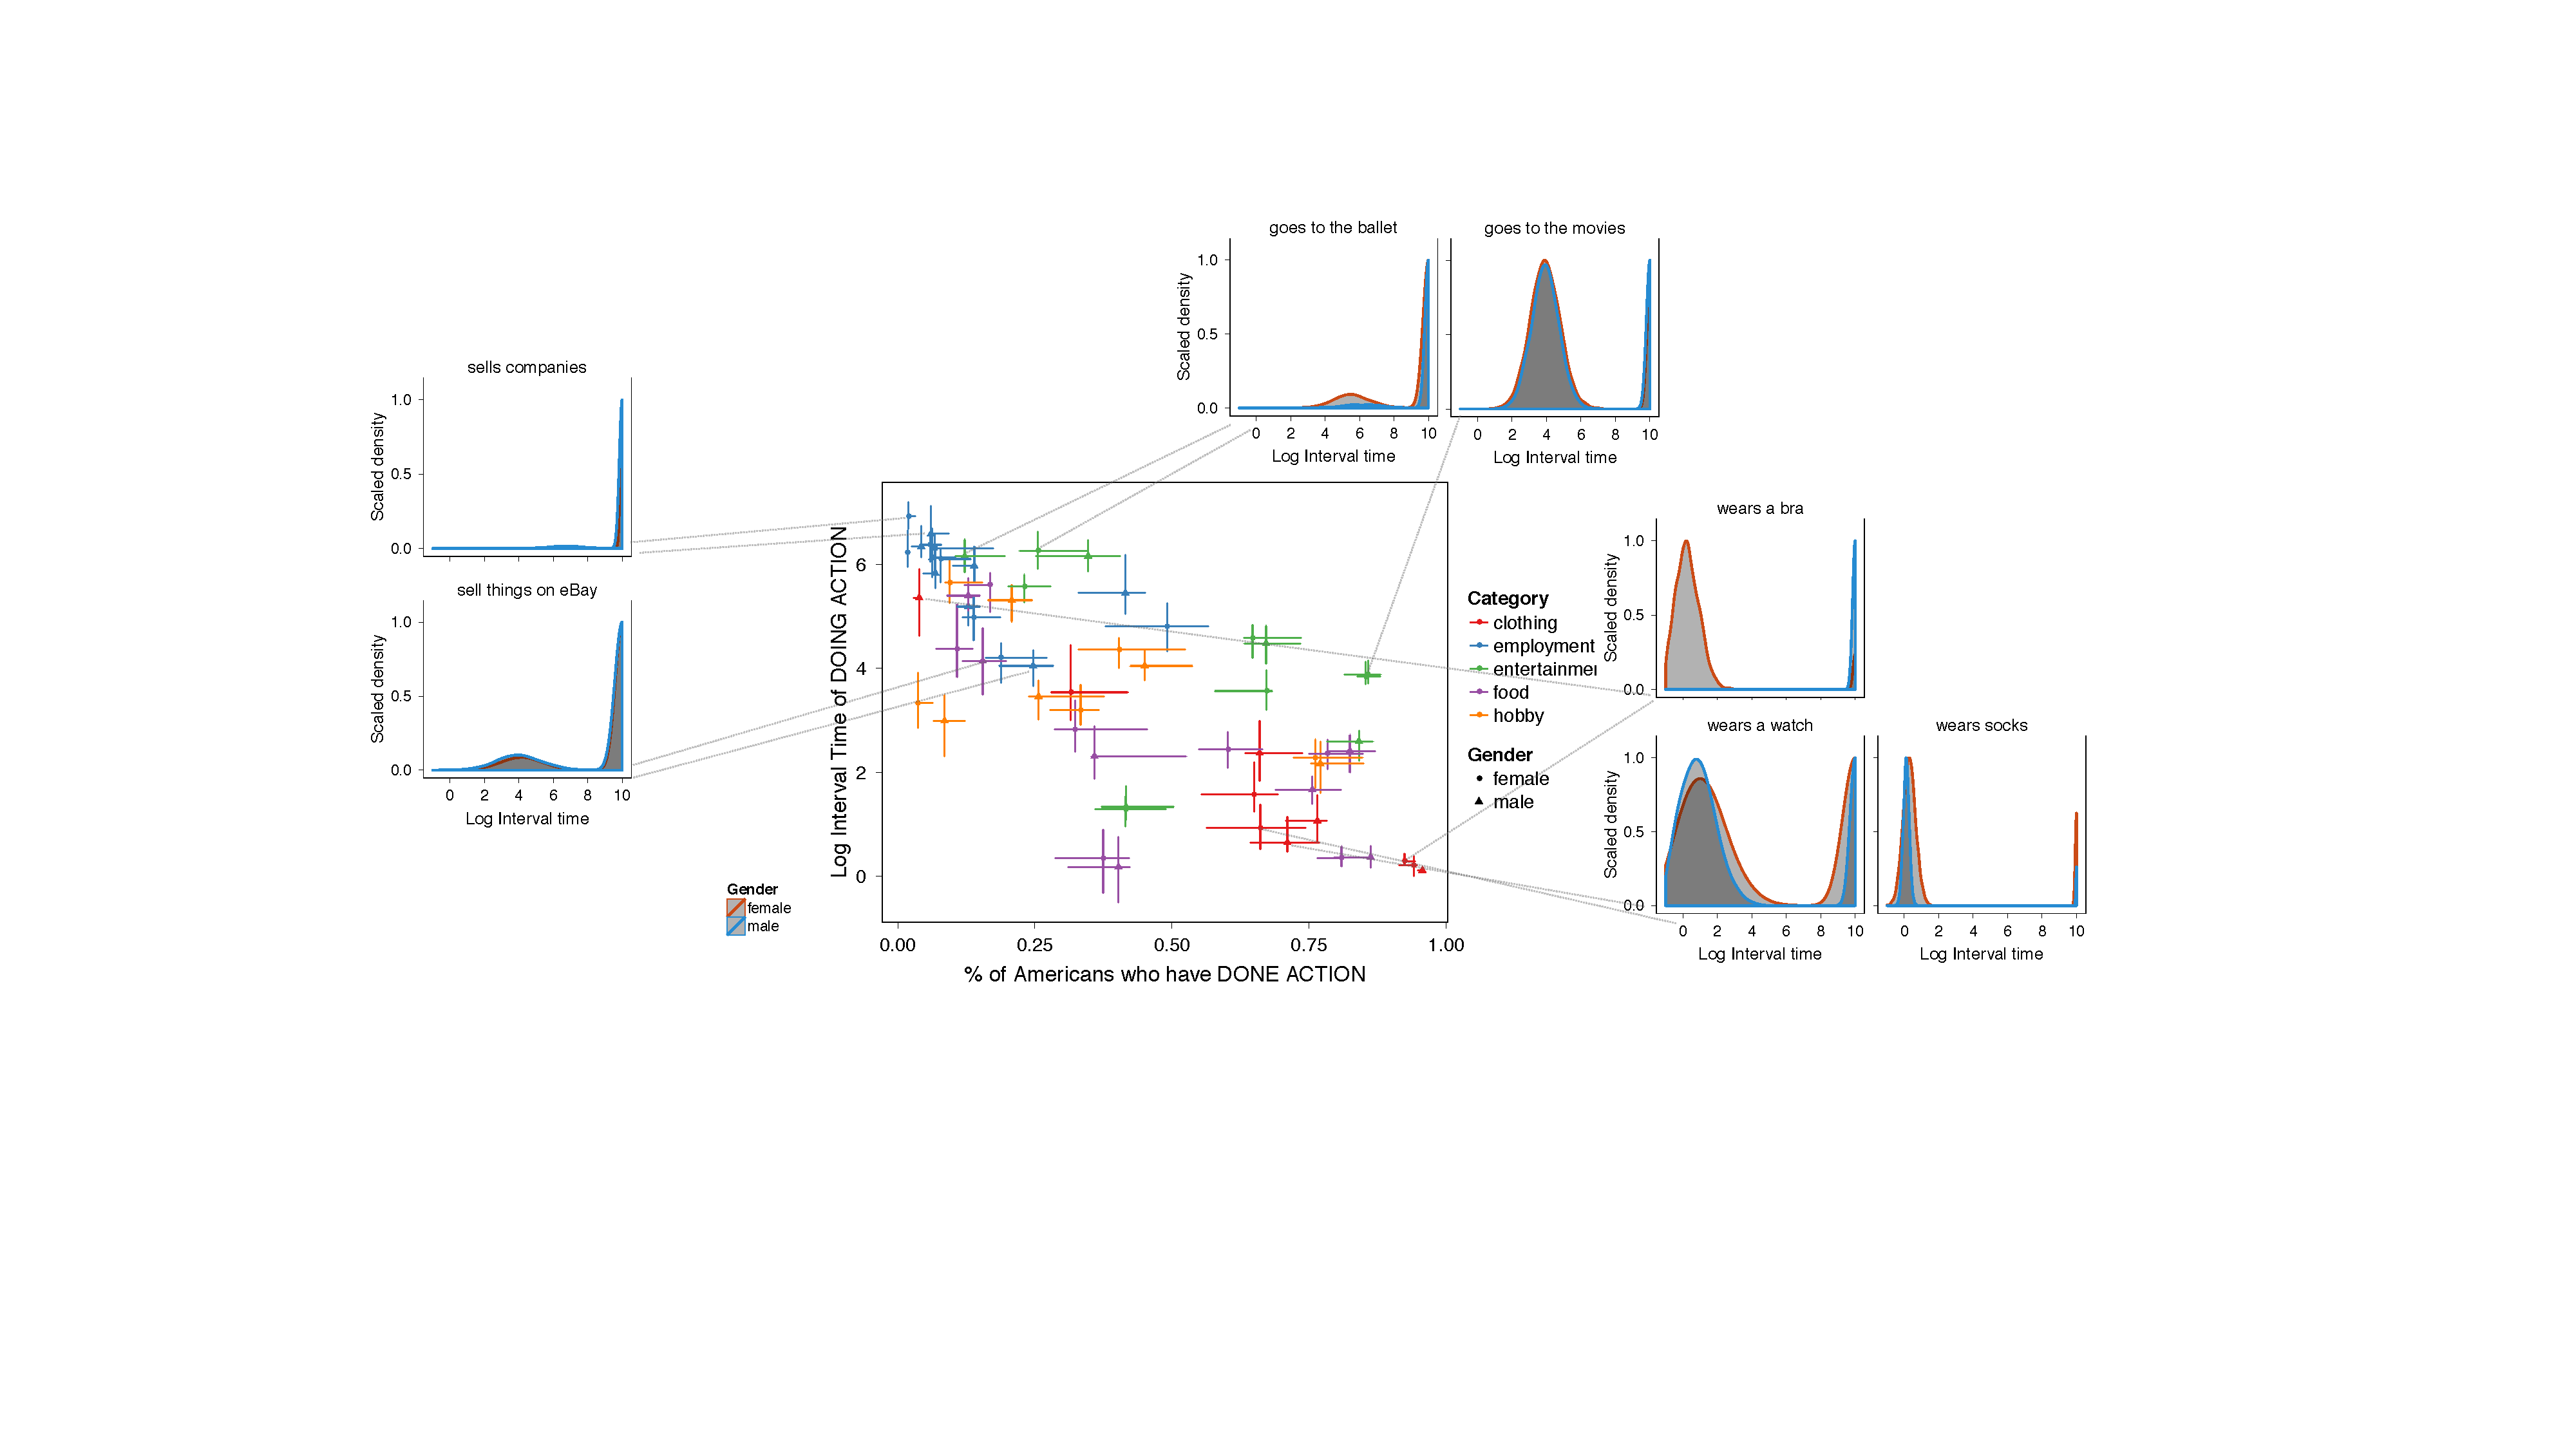
\includegraphics[width=\textwidth]{prior-scatter-insets}
  \caption{}
  \label{fig:priorScatter}
\end{figure*}
%


\section{Experiment 1: Prior elicitation}

%Experiment 1 set out to empirically verify the long-held belief that habitual sentences are analogous to generic sentences about events. 
%We used an adapted version of the computational model presented by \citeA{TesslerUnderReview} to guide the experimental design.
%


%\subsection{Expt.~1a: prior elicitation}

\citeA{TesslerUnderReview} found that participants' beliefs about the prevalence of a property is structured as the result of a mixture distribution composed of kinds with the potential to have the property present and kinds that lack the potential to have the property present.
The prior distribution, thus, is modeled as a mixture distribution between these two possibilities \cite{Griffiths2005}, similar in spirit to Hurdle Models of epidemiological data \cite{hurdleModels}.

Here, we explore this hypothesis with respect to participants beliefs about the frequency with which people partake in various events or actions.


\subsection{Method}

\subsubsection{Participants}
We recruited 40 participants from Amazon's Mechanical Turk.
Participants were restricted to those with U.S. IP addresses and who had at least a 95\% work approval rating.
The experiment took on average 12 minutes and participants were compensated \$1.25 for their work.


\subsubsection{Procedure}

For each event, participants were asked two questions:
\begin{enumerate}
\item X out of every 1000 \{men, women\} has \textsc{done action} before.
\item For a typical \{man, woman\} who has \textsc{done action} before, how frequently does he or she \textsc{do action}? 
\end{enumerate}

Question (1) had a response format of entering a number, and participants were free to make the comparison number larger (default: 1000) should the event be more rare than 1 out of 1000.
Question (2) had a response format of entering a number of instances out of the time period of a year (by default). Participants were free to change the time period to week, month, or 5 years.
We expected there might be different beliefs about the frequency of events depending on whether the actor is male or female, so we asked about both genders. Participants answered both questions for each gender on each slide (4 questions total, order of male / female randomized between-subjects).
The experiment in full can be viewed at \url{http://stanford.edu/~mtessler/habituals/experiments/priors/priors-2.html}.

\subsubsection{Materials}

We used 31 events organized into minimal pairs or triplets from 5 different conceptual categories: food and drug (e.g. \emph{eats caviar}, \emph{eats peanut butter}), work (e.g. \emph{sells things on eBay}, \emph{sells companies}), clothing (e.g. \emph{wears a suit}, \emph{wears a bra}), entertainment (e.g. \emph{watches professional football}, \emph{watches space launches}) and hobbies (e.g. \emph{runs}, \emph{hikes}). 
Items were chosen to intuitively cover a range of likely frequencies of action, as well as to provide a minimal comparison to another item.

\begin{figure*}[t]
\centering
  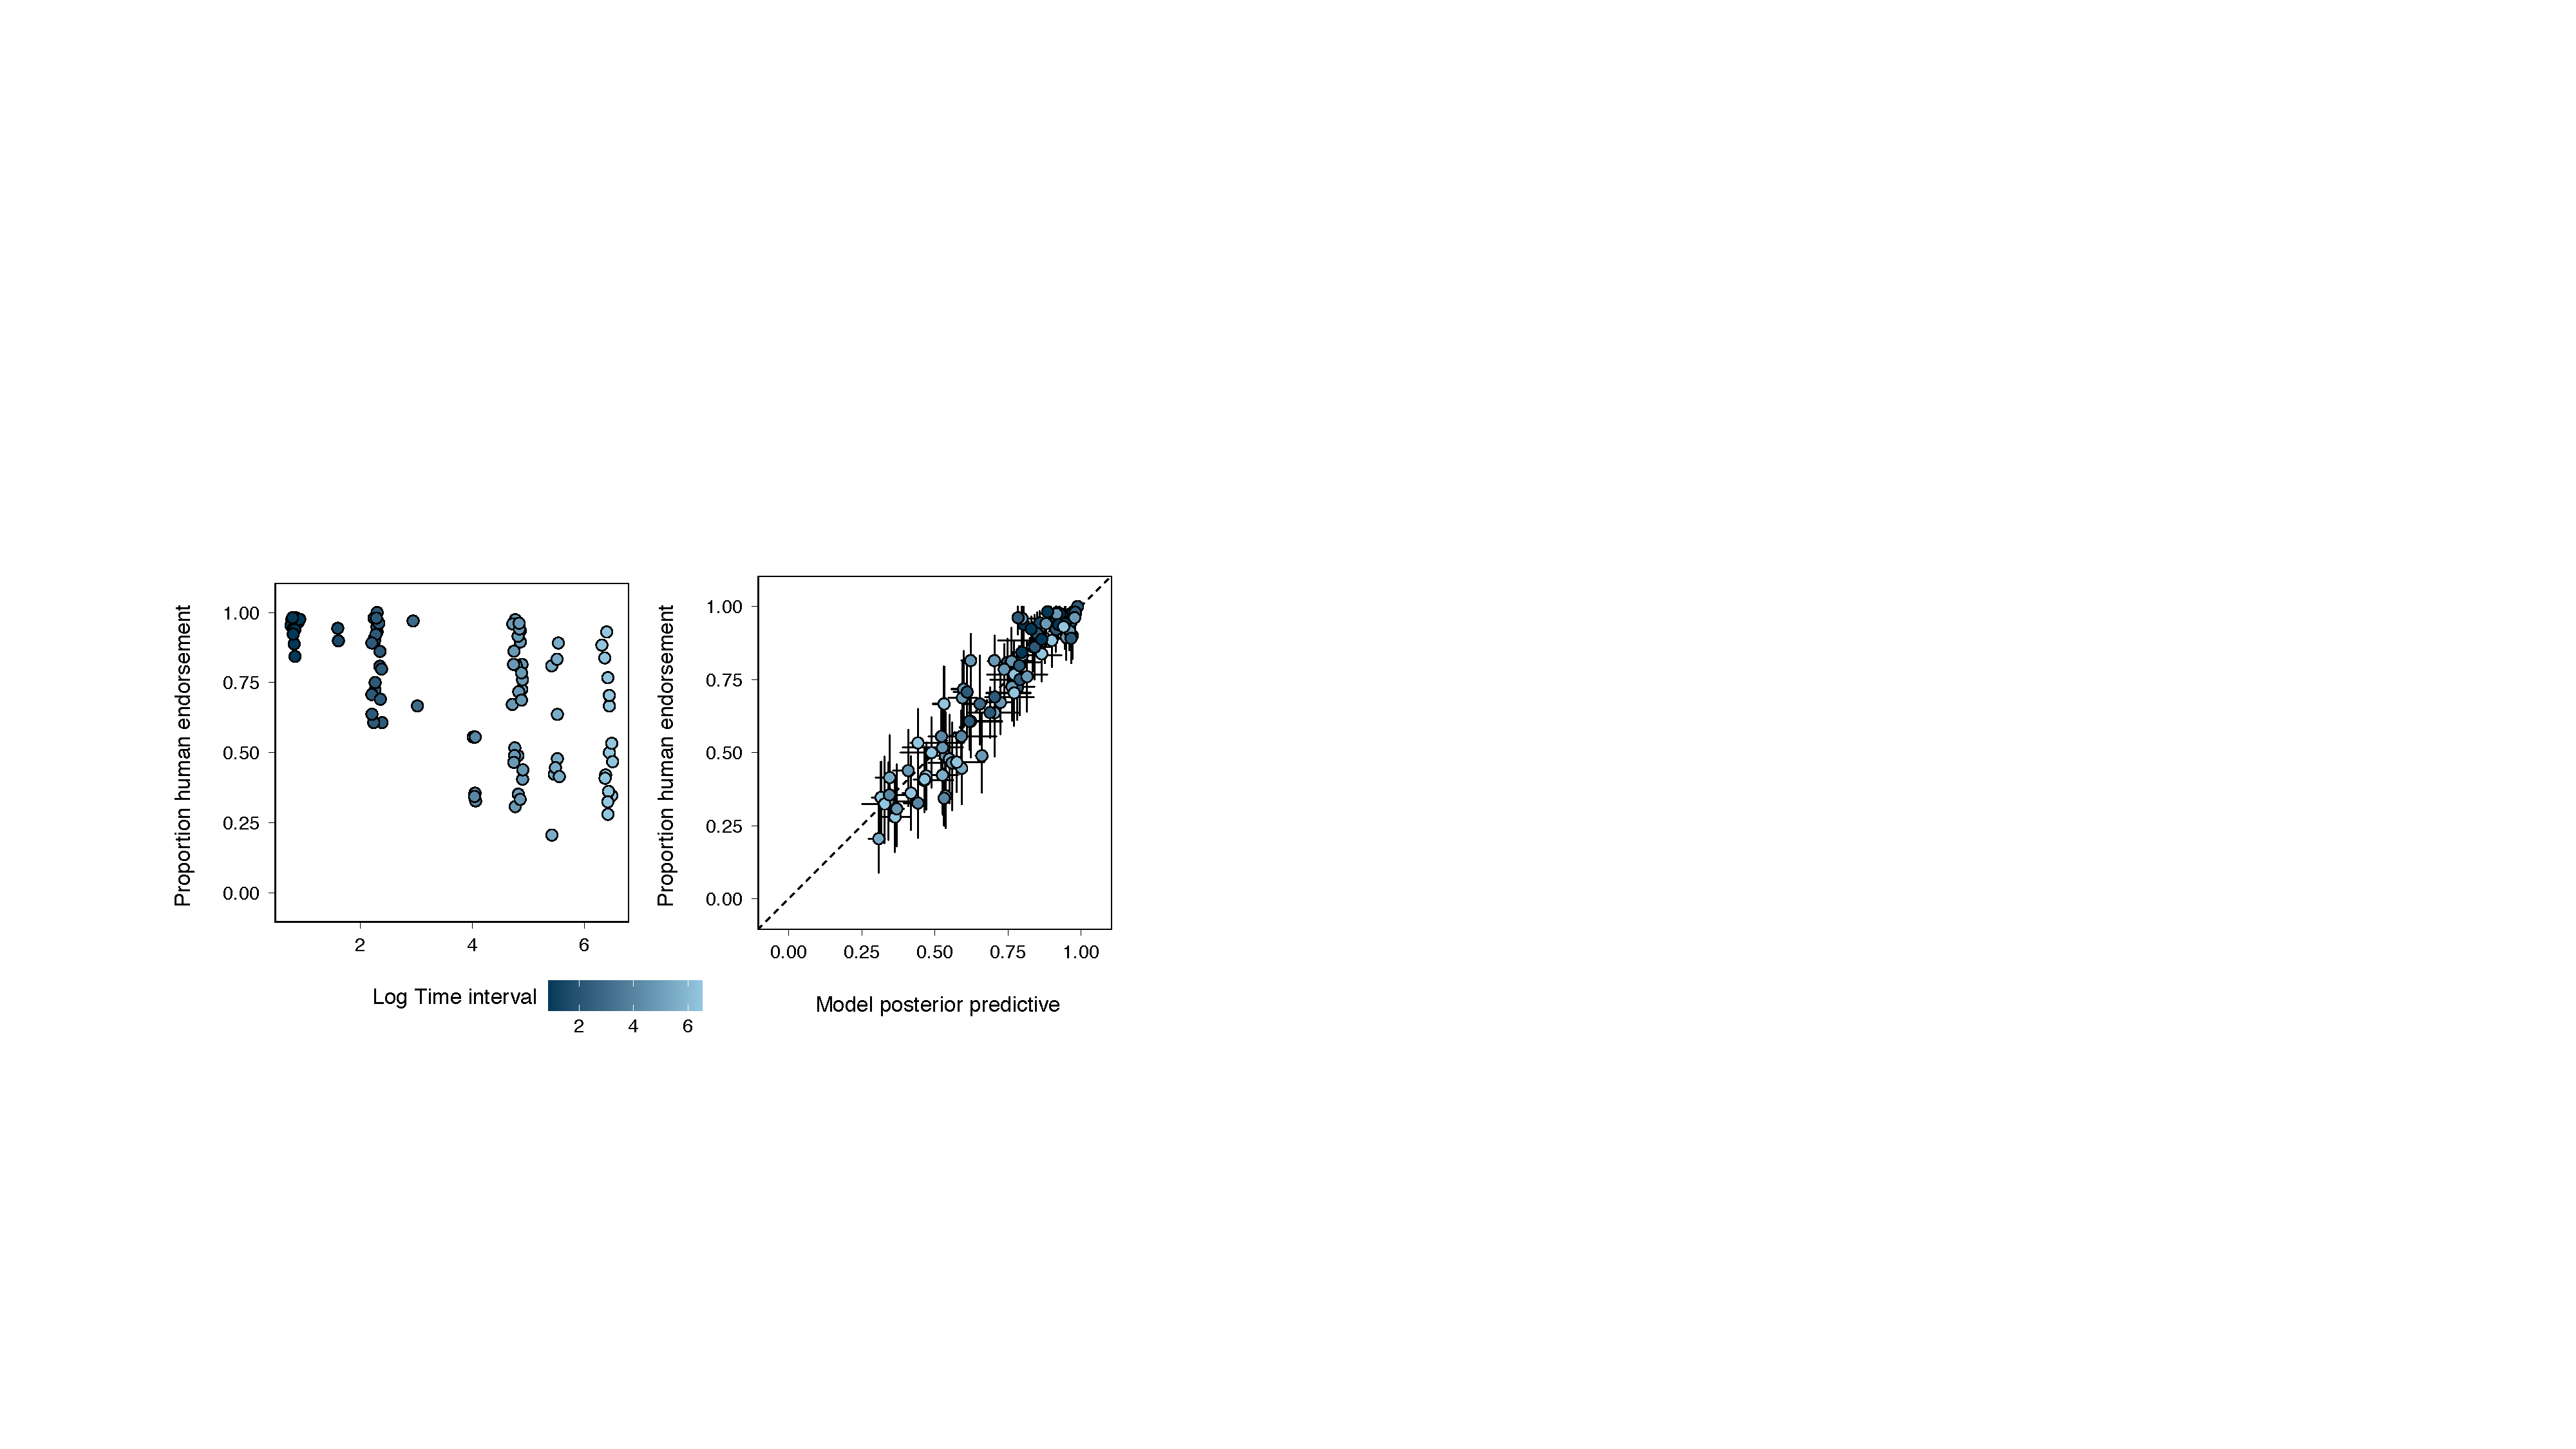
\includegraphics[width=\textwidth]{tj-scatters1}
  \caption{}
  \label{fig:tjScatters}
\end{figure*}


\subsection{Data analysis and results}

We modeled the data from question (1) as coming from a Beta distribution. 
Question (2) was modeled by a log-normal distribution. 
Each item was modeled independently.
%
\begin{minipage}{0.5 \textwidth} \small
\begin{align*}
d_{1} &\sim \text{Beta}(\gamma_{1}, \xi_{1}) \\
\ln d_{2} &\sim \text{Gaussian}(\mu_{2}, \sigma_{2}) \\
\end{align*}
\end{minipage}
%
We implemented this model using the probabilistic programming language WebPPL \cite{dippl}, and we learned about the credible values of the parameters and the posterior predictive distributions of the data by running MCMC using a variant of the Metropolis-Hastings algorithm.
%


The priors elicited indeed cover a range of possible parameter values (Figure \ref{fig:priorScatter}, scatter), resulting in parametrized distributions of dramatically different shapes (insets).  
We do observe a correlation in our items between the mean \% of Americans who have \textsc{done action} before (Question 1) and the mean log-interval time between actions (Question 2) ($r_{1,2} = -0.75; r^2_{1,2} = 0.55$); our items that tend to be more popular actions also tend to be more frequent actions (e.g. \textsc{wears socks}) and visa-versa (e.g. \textsc{steals cars}), though there are notable exceptions (e.g. \textsc{plays the banjo} is not popular but done frequently, as is \textsc{smokes cigarettes}; \textsc{goes to the movies} is a popular activity though not done very often). 

This diversity is relevant because the speaker model (Eq.~\ref{eq:S2}) will produce habitual sentences (e.g. \emph{Sam goes to the movies / goes to the ballet.}) contingent on the shape of the prior distribution. 
The posterior predictive distributions reconstruct the experimental data reasonably well for both question 1 ($r^2_{1} = 0.86$) and question 2 ($r^2_{2} = 0.68$); we use these parameterized priors going forward.


\section{Experiment 2: felicity judgments}

\subsection{Method}

\subsubsection{Participants}

We recruited 150 participants from MTurk.
The experiment took 4 minutes on average on participants were compensated \$0.55 for their work.

\subsubsection{Procedure and materials}

On each trial, participants were presented with a past frequency statement for a given action; the available actions were the same as in Expt. ~1a. 
The frequency statement was of the form: ``In the past N \{weeks, months, years\}, \textsc{person} has \textsc{done action} 3 times''.
We kept constant the number of times the action was done (3 times) in order to isolate the effects of the time window. 
The particular intervals used (number N and window \{weeks, months, years\}) were selected for each item to explore a wide range of predictions of the speaker model (Eq.~\ref{eq:S2}).

Participants were asked whether they agreed or disagreed with the corresponding habitual sentence: ``\textsc{person does action}''.
We identified 6 items for which the priors for men and women varied substantially in Expt.~1b.
We presented these items with both a male and a female name (on different trials) to explore the hypothesis that the comparison class against which the target person's behavior is compared is gender-specific (e.g. if there is a frequency at which a male would be judged to (habitually) \textsc{wear a bra} but a woman would not be judged to). 
The experiment in full can be viewed at \url{http://stanford.edu/~mtessler/habituals/experiments/truth-judgments/tj-2.html}.

%The model predicts that some items would not exhibit variability in endorsements in given ranges (e.g. if a person stole a car 3 times in the past \emph{week} vs. \emph{month}); we omitted particular intervals when the model predicted non-meaningful differences in endorsements. 

%\subsubsection{Materials}

\subsection{Behavioral results}

On each trial of the experiment, the participant was told a person did a particular action 3 times during some time window. 
Figure \ref{fig:tjScatters} (left) shows the correspondence between the time window given and the felicity of the corresponding habitual sentence. 
According to our theory that the meaning is a threshold of frequency of action, habitual sentences express minimally that a person \emph{has done} an action a number of times in the past. 
We see that none of our items receive less than 25\% endorsement (i.e. 75\% of participants disagree with the felicity of the utterance).
This may be due to the fact that actor has done the action in the past; we would expect to get strong disagreement with the utterance (endorsement = 0\%) when the person has never done the action, or done it only once.

As a baseline hypothesis, we see how the frequency of action predicts the felicity of a habitual sentence (e.g. how often John runs to predict the felicity of the sentence \emph{John runs}.). 
It is clear that a habitual sentence can receive strong agreement even when the actions are very infrequent (log time interval $>$ 4; time interval of subsequent actions years or more; e.g. writing 3 novels, stealing 3 cars in a 5 year interval).
We also see habitual sentences that participants are reluctant to endorse completely (e.g. wears socks, drinks coffee), even when they are relatively frequent in occurrence (spec. 3 times in a one month interval).
In our data, actions that are completed multiple times in a very short interval (spec, 3 times in a one week interval) receive at least 75\% endorsement, though there is still variability among them (e.g. smoking cigarettes, wearing socks are endorsed the least), suggesting that even actions that are completed almost everyday.



Overall, the time interval predicts only a fraction of the variability in responses ($r^2(93) = 0.33$).
For actions that are done on the time scale of years or more (upper median of time interval), time interval itself no longer explains the endorsements  ($r^2(50) = 0.07$)


\subsection{Model fit and results}

We used the posterior predictive of the prior data (Expt.~1a) as  $P(x)$  in Eq.~\ref{eq:S2} to predict felicity judgments in Expt.~1b.
We modeled $P(x)$ as a mixture of individuals with the possibility of carrying out the action and those without the possibility of doing it. 
The mixture component $\theta$ was determined by the frequency of people who had done the action before (Expt.~1a; Question 1, $d_1$). 
For those with the possibility of doing it, the frequency with which they carried out the action was modeled by a log-normal distribution, with parameters learned from the responses to Question 2. 

\begin{minipage}{0.5 \textwidth} \small
\begin{align*}
\theta & \sim \text{Beta}(\gamma_{1}, \xi_{1}) \\ 
\ln x & \sim \begin{cases} 
		\text{Gaussian}(\mu_{2}, \sigma_{2}) &\mbox{if } \text{Bernoulli}(\theta) = \textsc{t} \\
				\delta_{x=\infty} &\mbox{if } \text{Bernoulli}(\theta) = \textsc{f} \\
		\end{cases} \\
\end{align*}
\end{minipage}

Having fit the prior empirically, the model was one parameter -- the speaker optimality parameter in Eq.~\ref{eq:S1}. 
Additionally, we include a data analytic parameter to model random guessing behavior; this provides a rough measure of how much variance is unexplained by the pragmatics model. 
We use Bayesian data analytic techniques to integrate out these parameters \cite{LW2014}, and compare the posterior predictive distribution of this model to the empirical data in Expt.~1b.

To attain credible values of the model parameters as well as the posterior predictive distribution over responses, we collected 3 MCMC chains of 30,000 iterations, discarding the first 15,000 iterations of each chain for burn in.
The Maximum A-Posteriori (MAP) value and 95\% highest probability density (HPD) interval for the speaker optimality parameter in Eq.~\ref{eq:S1} is 4.7 [3.7,5.2].
The MAP and HPD interval for the data-analytic guessing parameter is 0.004 [0.0003, 0.03], suggesting that there is not a substantial amount of the data that is better explained by a model of random guessing than by the pragmatic speaker model.


The probabilistic pragmatics model does a better job of accounting for the variability in responses ($r^2(93) = 0.89$), including actions done on the time scale of years or more  ($r^2(50) = 0.89$) (Figure \ref{fig:tjScatters} right).


\section{Experiment 3: Time and subjective frequency}

In Expt.~1 \& 2, we saw how a model designed to describe generic language (e.g. \emph{Swans are white.}) can describe habitual language (e.g. \emph{John smokes}) equally as well by specifying the underlying degree as the frequency with which an individuals performs an action.
This provides a formal bridge between generalizations of properties about categories (i.e. \emph{generics}) and generalizations about individuals or events (i.e. \emph{habituals}), a connection often noted in the linguistics literature \cite{Carlson1977, Carlson2005, Cohen1999}. 

Unlike natural kinds, however, individuals can modify their behaviors overnight.  
In Expt.~3, we explore how knowledge of certain causal factors (e.g. the decision to retire; breaking one's leg) interacts with the frequency of action to modulate the veracity of habitual sentences (e.g. \emph{John writes novels.}; \emph{John runs.}).

These results suggest the underlying scale for habituals is \emph{predictive} frequency of action, and that habituals are used to talk about future predictions of people's actions.

\subsection{Method}

\subsubsection{Participants} 

We recruited \red{N} participants from MTurk.
The experiment took \red{N} minutes on average on participants were compensated \$\red{N} for their work.

\subsubsection{Procedure and materials}

The procedure was identical to Expt.~1b except for the inclusion of additional information on a subset of trials. 
On one third of the trials, participants were presented with \textbf{preventative conditions} (e.g. \emph{Yesterday, Bill decided to quit smoking.} that aimed to decrease the acceptability of the habitual sentence (\emph{Bill smokes}) even in the face of strong past frequency evidence (\emph{Last week, Bill smoked 3 times.}).
On one third of the trials, participants were presented with \textbf{enabling conditions} that were the same for all items (\emph{Yesterday, Bill remembered how much that was and made a plan to do it more in the future}) that aimed to increase the acceptability of the habitual sentence when the past frequency evidence was not strong. 
The final third of trials had no additional evidence and were identical to Expt.~1b. 
The dependent measure was the same as in Expt.~1b. 
The experiment in full can be viewed at \url{http://stanford.edu/~mtessler/habituals/experiments/truth-judgments/tj-3-preventative.html}.


\subsection{Behavioral results}

\subsection{Model results}



\section{Discussion}


Habitual sentences (e.g. \emph{Bill smokes}) express generalizations about events in an analogous way to how generic sentences (e.g. \emph{Swans are white.}) express generalizations about properties within categories. 
Though this connection has been pointed to in the philosophy and linguistics literatures, this work represents the first empirical and computational evidence unifying these two kinds of common, simple utterances. 
We also delved deeper into the semantics of these sentences, investigating the nature of the underlying frequency scale by introducing enabling and preventative conditions for the event to happen in the future. 
Future, or \emph{predictive}, frequency was shown to be extremely relevant in the truth conditions of habitual sentences. 

The pragmatic theory introduced by \citeA{TesslerUnderReview} 

The habitual sentences we explored were all presented in the simple, present tense.
Generalizations can also occur in the past tense (e.g. \emph{Bill smoked}, or \emph{Bill used to smoke.}) and in the future tense (e.g. \emph{Bill will smoke}). 
The present tense is interesting because it is \emph{a priori} unclear when, in fact, the sentence is making reference to.  

In the psychological literature, habituals have received relatively little attention compared to their category counterpart \emph{generics}. 

\begin{enumerate}
\item Tense (past vs future vs present)
\item Methodological implications (using habituals as opposed to generics)
\item Contrast class (men vs women)
\end{enumerate}

\bibliographystyle{apacite}

\setlength{\bibleftmargin}{.125in}
\setlength{\bibindent}{-\bibleftmargin}

\bibliography{habituals-cogsci2016}


\end{document}
